\chapter{TLU Hardware}\label{ch:hardware}
Board \brd is an evolution of the miniTLU designed at the \gls{uob}. The board shares a few features with the miniTLU but also introduces several improvements. This chapter illustrates the main features of the board to provide a general view of its capabilities and an understanding of how to operate it in order to communicate with the \gls{dut}s.

\section{Inputs and interfaces}\label{ch:hwDUT}
\subsubsection{FMC}
The board must be plugged onto a \gls{fmc} carrier board with an \gls{fpga} in order to function correctly. The connection is achieved using a low pin count \gls{fmc} connector. The list of the pins used and the corresponding signal within the \gls{fpga} are provided in appendix at page~\pageref{ch:appendix}.\\

\subsubsection{Device under test}\label{ch:dut}
The \gls{dut}s are connected to the \gls{tlu} using standard size \gls{hdmi} connectors\footnote{In the miniTLU hardware there were mini\gls{hdmi} connectors.}.\\
In the current version of the hardware, up to four \gls{dut}s can be connected to the board. In this document the connectors will be referred to as \verb|HDMI1|, \verb|HDMI2|, \verb|HDMI3| and \verb|HDMI4|.\\
The connectors expect 3.3~V \gls{lvds} signals and are bi-directional, i.e. any differential pair can be configured to be an output (signal from the TLU to the DUT) or an input (signals from the DUT to the TLU) by using half-duplex line transceivers. Figure~\ref{fig:LVDSTransceiver} illustrates how the differential pairs are connected to the transceivers.
\begin{alertinfo}{Note}
    The input part of the transceiver is configured to be always on. This means that signals going \emph{into} the \gls{tlu} are always routed to the logic (\gls{fpga}). By contrast, the output transceivers have to be enabled and are off by default: signal sent from the logic to the \gls{dut}s cannot reach the devices unless the corresponding enable signal is active.
\end{alertinfo}
Table~\ref{tab:HDMIpins} shows the pin naming and the corresponding output enable signal. The clock pairs have two different enable signals to select the clock source (see section~\ref{ch:clock} for more details). In general only one of the clock sources should be active at any time.\\
The enable signals can be configured by programming two \gls{gpio} bus expanders via \gls{i2c} interface as described in section~\ref{ch:i2c}.
 \begin{table}[]
    \centering
    \caption{HDMI pin connections.}
    \label{tab:HDMIpins}
    \begin{tabular}{|l|l|l|}
    \hline
    \textbf{HDMI PIN} & \textbf{HDMI Signal Name} & \textbf{Enable Signal Name} \\ \hline
     &  &  \\ \hline
    1   & \verb|HDMI_CLK| & \begin{tabular}[c]{@{}l@{}}\verb|ENABLE_CLK_TO_DUT|\\ or\\ \verb|ENABLE_DUT_CLK_FROM_FPGA|\end{tabular} \\ \hline
    2   & \verb|GND|       & -- \\ \hline
    3   & \verb|HDMI_CLK| * & \begin{tabular}[c]{@{}l@{}}\verb|ENABLE_CLK_TO_DUT|\\ or\\ \verb|ENABLE_DUT_CLK_FROM_FPGA|\end{tabular} \\ \hline
    4   & \verb|CONT|      & \verb|ENABLE_CONT_FROM_FPGA| \\ \hline
    5   & \verb|GND|       & -- \\ \hline
    6   & \verb|CONT*|     & \verb|ENABLE_CONT_FROM_FPGA| \\ \hline
    7   & \verb|BUSY|      & \verb|ENABLE_BUSY_FROM_FPGA| \\ \hline
    8   & \verb|GND|       & -- \\ \hline
    9   & \verb|BUSY*|     & \verb|ENABLE_BUSY_FROM_FPGA| \\ \hline
    10  & \verb|SPARE|     & \verb|ENABLE_SPARE_FROM_FPGA| \\ \hline
    11  & \verb|GND|       & -- \\ \hline
    12  & \verb|SPARE*|    & \verb|ENABLE_SPARE_FROM_FPGA| \\ \hline
    13  & n.c.      &  \\ \hline
    14  & \verb|HDMI_POWER| & -- \\ \hline
    15  & \verb|TRIG|      & \verb|ENABLE_TRIG_FROM_FPGA| \\ \hline
    16  & \verb|TRIG*|     & \verb|ENABLE_TRIG_FROM_FPGA| \\ \hline
    17  & \verb|GND|       &  \\ \hline
    18  & n.c.      &  \\ \hline
    19  & n.c.      &  \\ \hline
    \end{tabular}
\end{table}
\begin{figure}
  \centering
  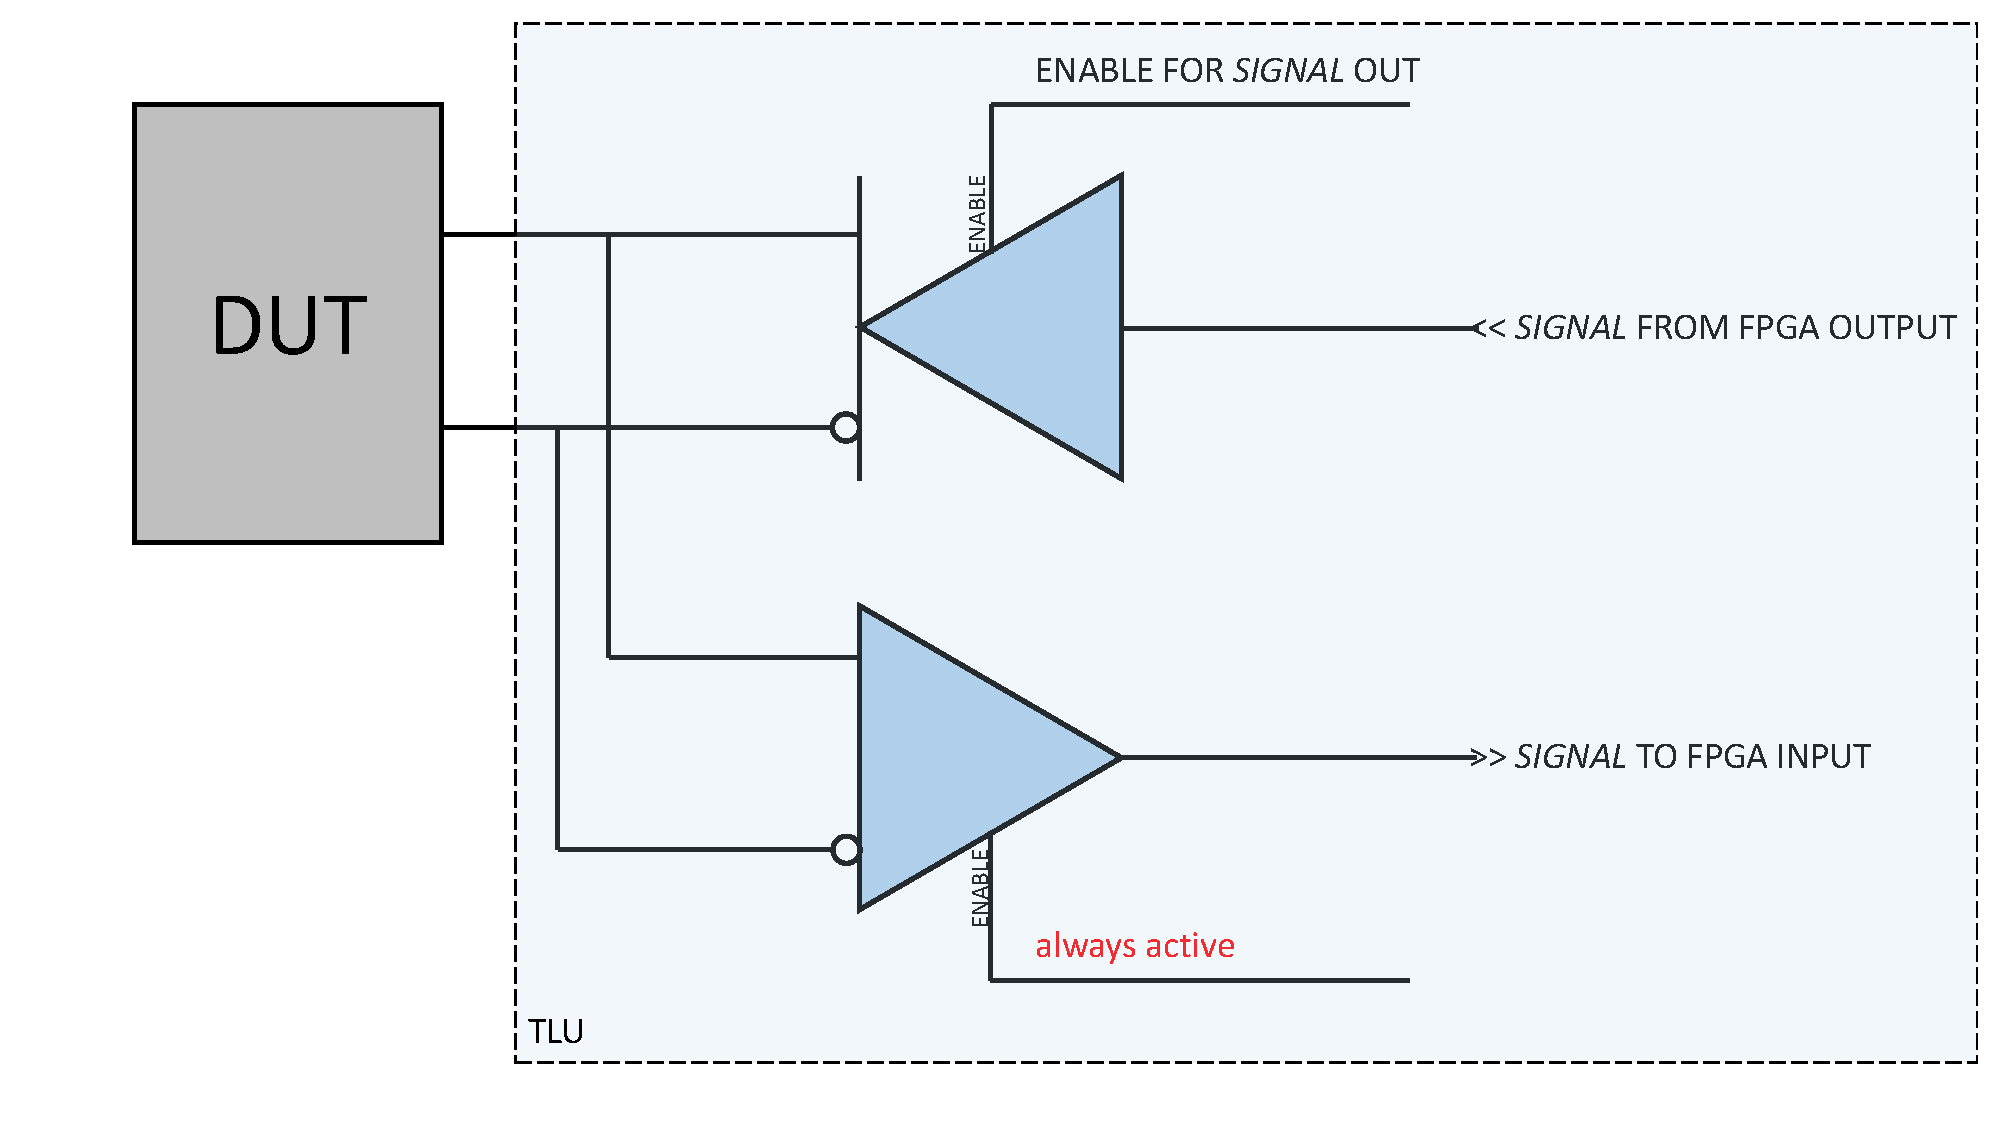
\includegraphics[width=.80\textwidth]{./Images/LVDS_transceiver.pdf}
  \caption{Internal configuration of the HDMI pins for the DUTs. The path from the DUT to the FPGA is always active. The path from the FPGA to the DUT can be enabled or disabled by the user.}\label{fig:LVDSTransceiver}
\end{figure}\\
In terms for functionalities, the four \gls{hdmi} connectors are identical with one exception: the clock signal from \verb|HDMI4| can be used as reference for the clock generator chip mounted on the hardware. For more details on this functionality refer to section~\ref{ch:clock}.

\section{Clock LEMO}
The board hosts a two-pin LEMO connector that can be used to provide a reference clock to the clock generator (see section~\ref{ch:clock}) or to output the clock from the \gls{tlu} to the external world, for instance to use it as a reference for another \gls{tlu}. The signal level is 3.3~V \gls{lvds}.\\
As for the differential pairs of the \gls{dut}s, the pins of this connector are wired to a transceiver configured to always accept the incoming signals. The outgoing direction must be enabled by using the \verb|ENABLE_CLK_TO_LEMO| signal, which can be configured using the bus expander described in in section~\ref{ch:i2c}.

\section{Trigger inputs}
Board \brd can accept up to six trigger inputs over the LEMO connectors labelled \verb|IN_1|, \verb|IN_2|, \verb|IN_3|, \verb|IN_4|, \verb|IN_5| and \verb|IN_6|. The \brd uses internal high-speed\footnote{500$\pm$30~ps propagation delay.} discriminators to detect a valid trigger signal. The voltage thresholds can be adjusted independently for each input in a range from -1.3~V to +1.3~V with 40~$\mu$V resolution.\\
The adjustment is performed by writing to two 16-bit \gls{dac}s via \gls{i2c} interface as described in section~\ref{ch:i2c}.\\
The \gls{dac}s can either use an internal reference voltage of 2.5~V or an external one of 1.3~V provided by the \gls{tlu}: it is recommended to choose the external one by configuring the appropriate register in the devices.\\
The correspondence between DAC slave and thresholds is shown in table~\ref{tab:DACOutputs}.
\begin{table}[]
\centering
\caption{DAC outputs and corresponding threshold inputs.}
\label{tab:DACOutputs}
\begin{tabular}{|l|c|c|}
\hline
                     & \multicolumn{2}{c|}{Output}                                                        \\ \hline
                     & \multicolumn{1}{l|}{\textbf{DAC2(Ic2)}} & \multicolumn{1}{l|}{\textbf{DAC1 (Ic1)}} \\ \hline
\textbf{Threshold 0} & 1                                       &                                          \\ \hline
\textbf{Threshold 1} & 0                                       &                                          \\ \hline
\textbf{Threshold 2} &                                         & 3                                        \\ \hline
\textbf{Threshold 3} &                                         & 2                                        \\ \hline
\textbf{Threshold 4} &                                         & 1                                        \\ \hline
\textbf{Threshold 5} &                                         & 0                                        \\ \hline
\end{tabular}
\end{table}


\section{I$^{2}$C slaves}\label{ch:i2c}
The \gls{i2c} interface on the \brd can be used to configured several features of the board.\\
Table~\ref{tab:I2C addresses} lists all the valid addresses and the corresponding slave on the board. The Enclustra lines refer to slaves located on the PM3 board; these slaves can be ignored with the exception of the bus expander. The Enclustra expander is used to enable/disable the \gls{i2c} lines going to the \gls{fmc} connector.
\begin{alertinfo}{Note}
    After a power cycle the Enclustra expander is configured to disable the \gls{i2c} interface pins. This means that it is impossible to communicate to any \gls{i2c} slave on the \gls{tlu} until the expander has been enabled.\\
    The interface is enable by setting bit 7 to 0 on register 0x01 of the Enclustra expander.
\end{alertinfo}
\begin{table}[]
    \centering
    \caption{I$^{2}$C addresses of the TLU. }
    \label{tab:I2C addresses}
    \begin{tabular}{|l|l|l|l|}
    \hline
    \textbf{CHIP} & \textbf{ID} & \textbf{FUNCTION}        & \textbf{ADDRESS} \\ \hline
    IC1           & AD5665RBRUZ & DAC1                     & 0x1F             \\ \hline
    IC2           & AD5665RBRUZ & DAC2                     & 0x13             \\ \hline
    IC5           & 24AA025E48T & EEPROM                   & 0x50             \\ \hline
    IC6           & PCA9539PW   & I2C Expander1            & 0x74             \\ \hline
    IC7           & PCA9539PW   & I2C Expander2            & 0x75             \\ \hline
    IC8           & ADN2814ACPZ & CDR                      & 0x60             \\ \hline
    IC8\_9        & Si5345A     & Clock Generator          & 0x68             \\ \hline
    \multicolumn{4}{|l|}{Enclustra slaves}                                                    \\ \hline
                  &             & Enclustra Bus Expander   & 0x21             \\ \hline
                  &             & Enclustra System Monitor & 0x21             \\ \hline
                  &             & Enclustra EEPROM         & 0x54             \\ \hline
                  &             & Enclustra slave          & 0x64             \\ \hline
\end{tabular}
\end{table}
Once the interface is enabled it is possible to read and write to the devices listed in the top part of table~\ref{tab:I2C addresses}.\\
The user should reference the manual of each individual component to determine the register that must be addressed. The rest of this section is meant to provide an overview of the slave functionalities.

\subsubsection{DAC}
Each \gls{dac} has four outputs that can be configured independently. \verb|DAC1| is used to configure the thresholds of the first four trigger inputs; \verb|DAC2| configures the remaining two thresholds.\\
The \gls{dac}s should be configured to use the \gls{tlu} voltage reference of 1.3~V. In these conditions, writing a value of 0x00000 to a \gls{dac} output will set the corresponding threshold to -1.3~V while a value of 0xFFFF will set it to +1.3~V.

\subsubsection{EEPROM}
The \gls{eeprom} located on the board contains a factory-set unique number, used to identify each \brd unequivocally. The number is comprised of six bytes written in as many memory locations.\\
The identifier is always in the form: \verb|0xD8 80 39 XX XX XX| with the top three bytes indicating the manufacturer and the bottom three unique to each device.

\subsubsection{Bus expander}
The expanders are used as electronic switched to enable and disable individual lines. Each expander has two 8-bit banks; the values of the bits, as well as their direction (input/output) can be configured via the \gls{i2c} interface. For the purpose of the \gls{tlu}, all the expander pins should be configured as outputs since they must drive the enable signals on the \gls{dut} transceivers.

\subsubsection{Clock and data recovery chip}
The \gls{cdr} is used in conjunction with the \gls{sfp} cage to recover data and clock from the incoming bit stream. The functionality has not yet been implemented in the firmware so the \gls{i2c} slave can be ignored for now.

\subsubsection{Clock generator}
The clock for \brd can be generated using various external or internal references (see section~\ref{ch:clock} for further details). In order to reduce any jitter from the clock source and to provide a stable clock, the board hosts a Si5345 clock generator that needs to be configured via \gls{i2c} interface.\\
The configuration involves writing $\thicksim$380 register values. A configuration file, containing all the register addresses and the corresponding values, can be generated using the ClockBuilder tool available from \href{http://www.enclustra.com/en/home/}{Silicon Labs}.\\
The registers addresses between 0x026B and 0x0272 contain user-defined values that can be used to identify the configuration version: it is advisable to check those registers and check that they contain the correct code to ensure that the chip is configured according to the \gls{tlu} specifications. As an indication, files generated for the current version of the \gls{tlu} should have a configuration identifier in the form \verb|TLU1E_XX|, where \verb|XX| is a sequential number.\\
\begin{alertinfo}{TLU Producer}
    When using the TLU producer to configure hardware, the location of the configuration file can be specified by setting the \texttt{CLOCK\_CFG\_FILE} value in the \emph{conf} file for the producer.\\
    If no value is specified, the software will look for the configuration file \texttt{../conf/confClk.txt} i.e. if the \texttt{euRun} binary file is located in \texttt{./eudaq/bin}, then the default configuration file should reside in \texttt{./eudaq/conf}. The configuration will produce an error if the file is not found.
\end{alertinfo}
